\chapter{Model-based testing}

\begin{quote}
``\emph{Program testing can be used to show the presence of bugs, but never to show their absence!}'' -- \textnormal{E. Dijkstra: {\em Notes On Structured Programming}, 1970.}
\end{quote}


This final chapter of the subject notes deals with testing in high integrity systems. Despite high-integrity software requiring quality assurance techniques that go far beyond testing, the tasks of designing and executing tests is still an integral part of the process.

In this chapter, we will look at one particular type of testing: \emph{model-based testing}. Model-based testing is the use of design models to design and/or execute tests. The formal nature of many methods used in high integrity systems provides advantages in testing far beyond what is capable in less formal environments.


\subsubsection*{Learning outcomes}

The learning outcomes of this chapter are:

\begin{enumerate}

 \item Systematically construct tests from formal models using the Test Template Framework.

 \item Apply adapted Test Template Framework to Alloy specifications.

\end{enumerate}


\section{Testing in high-integrity systems}


Given what we have learnt so far regarding program proofs, and Dijkstra's famous quote at the start of the chapter, the following question seems pertinent: \emph{what place does testing have in high-integrity systems engineering?}

Despite the use of more formal methods to prove properties about our programs, testing is still required for several reasons, including:

\begin{enumerate}

 \item To find problems that escape detection earlier in the project lifecycle. For example, if we make the same incorrect assumptions in both our contract and our program, tools like the SPARK tool chain may fail to find problems related to these assumptions. Testing may find these problems for us.

 \item To find problems related to the environment. Even if we can be 100\% confident that our program is logically correct, unexpected events in the environment, or problems related to the platform on which the software runs, may result in system failures. Testing is one way to help find these problems.

 \item To validate the system. If we take our formal specification, translate to a correct and complete design, and then implement that correctly, testing is still useful to validate that we built the right system. In other words, it is still useful for validating that our specification is correct and complete.

\end{enumerate}

\subsection{Systematic testing}

There are three general approaches we can take to testing:

\begin{enumerate}

 \item {\em Ad-hoc testing}, which is:

   \begin{enumerate}
     \item  ineffective: too late to influence design decisions; and

       \item expensive: testing is not reused properly to help with          product maintenance.

   \end{enumerate}

 \item \emph{Exploratory testing}, which  is:

   \begin{enumerate}
    \item creative: tests are designed ``on the fly'', so that new tests are being run all the time; and
    \item lightweight: tests are not pre-prepared, and are often not documented.
   \end{enumerate}


 \item {\em Systematic testing}, which is:

   \begin{enumerate}

     \item planned: allows designing for testability;
     \item documented: tests can be reviewed, understood, and evaluated; and
     \item maintained: tests are executed after every change (known as {\em regression testing}).

   \end{enumerate}

\end{enumerate}

For high-integrity software, exploratory testing is highly effective, and systematic testing is imperative. In this chapter, we will look only at systematic model-based testing, and a technique for model-based testing that forms the basis of many modern model-based testing tools.


There are three broad steps in systematic testing:

\begin{description}
 \item[Planning:]~

  \begin{itemize}
 
    \item Provide test scaffolding such as drivers and stubs.

    \item Create test inputs.

    \item Derive expected outputs for those inputs.

  \end{itemize}


 \item[Execution:]~

  \begin{itemize}
 
    \item Execute test cases and capture actual outputs.
    
  \end{itemize}

\item[Evaluation:]~

  \begin{itemize}
 
    \item Compare actual and expected outputs.
  
   \item Report findings.

\end{itemize}
\end{description}

Model-based testing can help to automated (or semi-automate) parts of these steps.

\section{Model-based testing}


\begin{definition}[Model-based testing]
Model-based testing is the use of design models for performing and executing artifacts related to the testing of systems. For example: automated test input generation, automatic stub generation, and automatic oracle generation.
\end{definition}

Models can be anything from simple data-flow models, to UML statecharts, to abstract mathematical specifications. In this subject, we will focus on using mathematical specifications (Alloy specification) to automatically generating test inputs and outputs. We will adapt the {\em Test Template Framework} \cite{stocks96}, which is the basis for many model-based testing methods and tools.

\begin{example}[The triangle program]
As a running example, we will use the triangle program proposed by Glenford Myers in {\em The Art of Software Testing} \cite{myers79}.

The program reads three integer values that are interpreted as the lengths of the sides of a triangle. The program returns a value indicating whether the triangle is equilateral, isosceles, scalene, or invalid.

\paragraph{Tests for the triangle program}

Myers suggests at least the following test inputs for the triangle program:

\begin{itemize}
 \item 1 valid scalene
 \item 3 valid isosceles (1 for each side being the odd one out)
 \item 1 valid equilateral
 \item one side with a 0
 \item all sides 0
 \item 3 permutations such that sum of two sides = third
 \item 3 permutations such that sum of two sides $<$ third
 \item negative side
 \item non-integers (if possible)

\end{itemize}
\end{example}

\begin{example}[The triangle program: A formal definition in Alloy]
In this example, we formally describe the triangle example in Alloy.

First, we declare the different types of triangle. A triangle can be either equilateral, isosceles, scalene, or invalid:

\lstset{aboveskip=3mm}
\alloyfile{linerange={3-3}}{\rootdir/ttf/models/triangle.als}

Then, we describe a predicate called $validTriangle$, which returns true if and only if three integers representing the length of sides form a valid triangle:

\lstset{aboveskip=3mm}
\alloyfile{linerange={5-7}}{\rootdir/ttf/models/triangle.als}

This concise definition is enough to determine whether three integers form a correct triangle, including negative integers.

Next, we define the valid and invalid triangle cases:

\lstset{aboveskip=3mm}
\alloyfile{linerange={9-19}}{\rootdir/ttf/models/triangle.als}


The specification for the invalid case is straightforward. For the valid case, we categorise the set of three inputs into three different cases. This uses the property of sets that states that each element only occurs once in a set. For example, the set \texttt{\{1,2,2\}} is equivalent to \texttt{\{1,2\}}, and further, the expression \texttt{\#\{1,2,2\}}, which denotes the size of the set, is 2. That is, the set \texttt{\#\{1,2,2\}} has only two elements: 1 and 2.


Using this property of sets, the valid case is split into three cases depending on the Alloy relation \texttt{(x+y+z)}\footnote{Recall that in Alloy, all sets are unary relations, and that \texttt{+} is the union operator.}: (1) the case in which the set has only one element (the three values are all equal); (2) the case in which the set has only two elements (two elements are equal); and (3) the case in which the set has three elements (all elements are non-equal).

Finally, these two predicates are brought together into a single predicate using the disjunction operator:

\lstset{aboveskip=3mm}
\alloyfile{linerange={21-23}}{\rootdir/ttf/models/triangle.als}

Thus, the inputs either form a valid or invalid triangle.
\end{example}



\section{The Test Template Framework (TTF)}

The Test Template Framework (TTF) \cite{stocks96} is one of the earliest model-based testing frameworks, and many model-based testing methods, tool, and frameworks, such as Smartesting's toolset, are based on it.

The TTF is based around the Z language, but this is its notation only. The general idea has wide applicability, as evidenced by the fact that most model-based testing frameworks built on this do not support models written in Z. We will apply it to Alloy models.

The idea behind the TTF is to systematically derive tests while also implicitly recording how those tests came about. That is, it considers testing to be more than just a statement about input data --- the functional behaviour specification, the test outputs, and test purpose are all important considerations that must be taken into account.

\subsection{Process}

Using the TTF, one takes a model-based specification and executes the following process:

\begin{enumerate}

 \item Identify the {\em input space} (IS),  {\em valid input space} (VIS), and {\em output space} (OS) of the program.

 \item Apply {\em test tactics} to partition the leaf nodes of a {\em testing tree}, with the VIS being the initial leaf node. This is a formalisation of the well-known \emph{equivalence partitioning} testing technique.

 \item Prune infeasible paths in the tree.

 \item Derive test inputs from the leaf nodes of the testing tree.

 \item Derive expected outputs for the test inputs.

\end{enumerate}

\subsection{Input spaces and output spaces}

The first step is to identify the input space, output space, and \emph{valid} input space.

\subsubsection*{Predicates as input and output spaces}

Before we define the input/output space formally, we introduce some shorthand notation (actually borrowed directly from Z). These are actually just horizontal definitions of normal Alloy predicates, as follows:

\lstset{aboveskip=3mm}
\begin{alloy}[escapeinside={++}]
 S == [+\emph{Pred}+ | +\emph{P}+]
\end{alloy}

This declares a new predicate \texttt{S} by extending an Alloy predicate \texttt{Pred} with new information in \texttt{P}. This is just a shorthand way of declaring the following:

\lstset{aboveskip=3mm}
\begin{alloy}[escapeinside={++}]
 pred S [+\emph{Variable Declarations from Pred}+] {
   +\emph{Predicate from Pred}+
   +\emph{P}+
 }
\end{alloy}

In the TTF, input and output spaces are declared as predicate. That is, an input/output space is a list of variable declarations specifying the space, and a predicate that constrains that space.

\begin{definition}[Input Space]
The TTF defines the input space as follows. Let \texttt{Op} be an Alloy predicate representing the operation under test. Let \texttt{x$_1$,\ldots,x$_n$} be all the input and non-primed state variables referenced in \texttt{Op}, and \texttt{T$_1$,\ldots, T$_n$} their corresponding types. The Input Space (IS) of \texttt{Op}, written \texttt{IS\_OP}, is the  predicate defined by:

\lstset{aboveskip=3mm}
\lstset{language=}
\begin{alloy}[escapeinside={++}]
 IS_OP == [x+$_1$+ : T+$_1$+; +\ldots+; x+$_n$+ : +T$_n$+]
\end{alloy}
\end{definition}



\begin{definition}[Valid Input Space]
The TTF defines the input space as follows. Let \texttt{Op} be an Alloy predicate representing the operation under test, and $pre($\texttt{Op}$)$ be the precondition of \texttt{Op}. The Valid Input Space (VIS) of \texttt{Op}, written \texttt{VIS\_OP}, is the predicate defined by:

\lstset{aboveskip=3mm}
\lstset{language=}
\begin{alloy}[escapeinside={++}]
 VIS_OP == [IS_OP | +$pre($Op$)$]
\end{alloy}
\end{definition}

The above states the \texttt{VIS\_OP} is the same as \texttt{IS\_OP}, with the additional constraint $pre($\texttt{Op}$)$ added to the predicate part.

\begin{definition}[Output Space]
The TTF defines the input space as follows. Let \texttt{Op} be an Alloy predicate representing the operation under test. Let \verb+x+$_1$\verb+,+\ldots\verb+, x+$_n$ be all the output and primed state variables referenced in \texttt{Op}, and \texttt{T$_1$,\ldots, T$_n$} their corresponding types. The Output Space (OS) of \texttt{Op}, written \texttt{OS\_OP}, is the predicate defined by:

\lstset{aboveskip=3mm}
\lstset{language=}
\begin{alloy}[escapeinside={++}]
 OS_OP == [x+$_1$+ : T+$_1$+; +\ldots+; x+$_n$+ : +T$_n$+]
\end{alloy}
\end{definition}



\begin{example}[The triangle program: IS, OS, and VIS]
\label{ex:ttf:triangle-is-vis-os}
In this example, we define the input space, output space, and valid input space to the triangle program.

The input space and the valid input space take the input and non-primed state variables. Because the program has no state, we take just the input variables:

\lstset{aboveskip=3mm}
\lstset{language=}
\begin{alloy}
 IS_Tri == [x, y, z : Int]
 VIS_Tri == [x, y, z : Int]
\end{alloy}

The valid input space is the same as the input space because the \texttt{Tri} operation has the precondition:

\quad \verb+validTriangle[x, y, z] or not validTriangle[x, y, z]+,

which is equivalent to \texttt{true}. 

If the program only accepted valid triangles as input --- that is, the program was just the \texttt{ValidCase} predicate ---, the input and valid input spaces would be:

\lstset{aboveskip=3mm}
\lstset{language=}
\begin{alloy}
 IS_ValidCase == [x, y, z : Int]
 VIS_ValidCase == [IS_ValidCase | validTriangle[x, y, z]]
\end{alloy}

The output space for the triangle program is all output and primed state variables. Because the program has no state, the output space is just the single output variable:

\lstset{aboveskip=3mm}
\lstset{language=}
\begin{alloy}
 OS_ValidCase == [class : Triangle]
\end{alloy}


\end{example}

\subsection{Test tactics and partitioning}

The next step in the framework is to \emph{partition} the valid input space into disjoint \emph{test classes}. The process for doing this is iterative, and the end result is a \emph{testing tree}: a tree in which each non-leaf node has been partitioned into its child nodes. The root of the testing tree is the VIS.

At each step of the process, we apply a \emph{strategy} to one of more of the leaf nodes in the tree. Applying a strategy to a node in the tree results in two or more new nodes, which are children of the node to which the strategy was applied. Further to this, the following must hold:

\begin{enumerate}

 \item The new child nodes must be \emph{disjoint} from each other. That is, there must be no possible combinations of inputs that are possible in more than one child.

 \item The union of the new child nodes must be equal to the parent node. That is, if an input is in the parent node, it must also be in one of the child nodes, as \emph{vice versa}.

\end{enumerate}

In this section, we present some of the main test tactics, and apply the relevant tactics to the Triangle program.

\subsubsection{Tactic: Cause-effect analysis (CE)}

Cause-effect analysis is a testing strategy that partitions the {\em output} space, based on equivalence classes.

\begin{example}
In the triangle program there is a clear partition based on the different outputs: \texttt{EQU, ISO, SCA,} and \texttt{INV}.

If we apply this to the VIS of the triangle program, we partition the VIS into four {\em disjoint} classes:

\lstset{aboveskip=3mm}
\lstset{language=}
\begin{alloy}
 CE_EQU == [VIS_Tri | validTriangle[x, y, z] and #(x+y+z) = 1]
 CE_ISO == [VIS_Tri | validTriangle[x, y, z] and #(x+y+z) = 2]
 CE_SCA == [VIS_Tri | validTriangle[x, y, z] and #(x+y+z) = 3]
 CE_INV == [VIS_Tri | not validTriangle[x, y, z]]
\end{alloy}
\end{example}

Note two important items of syntax/documentation here:

\begin{enumerate}

 \item The prefix \texttt{CE} to the predicate names refers to ``cause-effect'' -- the strategy being used, and documents the tactic that was used to generate this class. The suffixes document the particular class; e.g.\ \texttt{EQU} documents that this is the equivalence class for equilateral.

 \item As with constructing the predicate \texttt{VIS\_Tri} in Example~\ref{ex:ttf:triangle-is-vis-os}, we again use predicates as declarations. Thus, the class \texttt{CE\_EQU} is represented as a predicate, which is defined as the predicate \texttt{VIS\_Tri}, but only with valid equilateral triangles. The predicate \texttt{VIS\_Tri} itself includes the predicate \texttt{IS\_Tri}.

 If we expand to the full definition, we have the following:

\lstset{aboveskip=3mm}
\lstset{language=}
 \begin{alloy}
CE_EQU == [x,y,z : Int | validTriangle[x,y,z] and #(x+y+z) = 1]
 \end{alloy}
\end{enumerate}


\subsubsection{Tactic: Partition analysis (PA)}

Partition analysis reduces the formal definition into {\em disjunctive normal form} (DNF), and extracts disjoint classes from the disjunction to form new child classes.

A proposition is in DNF if and only if it is a disjunction (\texttt{or}) of one or more conjunctions (\texttt{and}), atomic propositions, or negations of atomic propositions. For example, \verb+A and (B or C)+ is not in DNF. We must translate it into DNF using De Morgan's laws: \verb+(A and B) or (A and C)+.

Using partition analysis, the predicate \verb+A or B+ would be treated as two separate partitions if they were disjoint. However, if \texttt{A} was not disjoint from \texttt{B}, then three partitions would be created instead: \verb+A and B+, \verb+not A and B+, and finally \verb+A and not B+.


\begin{example}
For the triangle example, we partition the four classes using the PA strategy. For the equilateral and scalene triangles, there are no partitions. For the isosceles case, there are three cases: one representing each of the three sides being the ``odd one out''. We can represent this using the predicate:

\begin{tabular}{lll}
 &          & \verb+(x = y and z != x) or+\\
 &          & \quad\verb+(x = z and y != x) or+\\
 &          & \quad\verb+(y = z and y != x)+
\end{tabular}

This predicate is in DNF, because it is a disjunction of atomic predicates. Further, it is disjoint. Thus, we can create three new disjoint classes from the parent:

\lstset{aboveskip=3mm}
\lstset{language=}
\begin{alloy}
 PA_ISO.1 == [CE_ISO | x = y and z != x]
 PA_ISO.2 == [CE_ISO | x = z and y != x]
 PA_ISO.3 == [CE_ISO | y = z and y != x]
\end{alloy}


For the class \texttt{CE\_INV}, first, we expand the definition of \verb+not validTriangle[x, y, z]+ and reduce to DNF:

\begin{tabular}{lll}
 &          & \verb|not (x < y + z and y < x + z and z < x + y)|\\
 & $\equiv$ & \verb|x >= y + z or y >= x + z or z >= x + y|
\end{tabular}

The first predicate above is a negation of a disjunction, so is not in DNF. We have to push the \texttt{not} operator into the disjunction, leaving the second predicate. This is a disjunction of atomic predicates, so is in DNF.

However, the predicate is not disjoint, because there are  values for the variables that satisfy more than one of the disjuncts; e.g.\ \verb+x = y = z = -1+. Therefore, we need to further partitioning using the rule above. This results in seven different permutations:

\lstset{aboveskip=3mm}
\lstset{language=}
\begin{alloy}
PA_INV.1 == [CE_INV | x >= y + z and y >= x + z and z >= x + y]
PA_INV.2 == [CE_INV | x <  y + z and y >= x + z and z >= x + y]
PA_INV.3 == [CE_INV | x >= y + z and y <  x + z and z >= x + y]
PA_INV.4 == [CE_INV | x >= y + z and y >= x + z and z <  x + y]
PA_INV.5 == [CE_INV | x <  y + z and y <  x + z and z >= x + y]
PA_INV.6 == [CE_INV | x <  y + z and y >= x + z and z <  x + y]
PA_INV.7 == [CE_INV | x >= y + z and y <  x + z and z <  x + y]
\end{alloy}

Using simple arithmetic, the first four classes can be simplified to:

\lstset{aboveskip=3mm}
\lstset{language=}
\begin{alloy}
PA_INV.1 == [CE_INV | x = 0 and y = 0 and z = 0]
PA_INV.2 == [CE_INV | x = 0 and y != 0 and y = z]
PA_INV.3 == [CE_INV | x != 0 and y = 0 and x = z]
PA_INV.4 == [CE_INV | x != 0 and x = y and z = 0]
\end{alloy}
\end{example}



\subsubsection{Tactic: Type-based selection (TB)}

This strategy is one that uses ``interesting values'' based on types. The term ``interesting values'' is somewhat subjective.

A good example is sets. If we have a set, an interesting value is the empty set ($\emptyset$), so we would choose one empty set and one non-empty set. If we have two sets, $S$ and $T$, we would choose the following permutations, based on set operators:

\begin{tabular}{lll}
  $S = \emptyset, T = \emptyset$ & &
    $S \neq \emptyset, T \neq \emptyset, S \subset T$  \\
  $S = \emptyset, T \neq \emptyset$ & & 
    $S \neq \emptyset, T \neq \emptyset, T \subset S$  \\
  $S \neq \emptyset, T = \emptyset$ & & 
    $S \neq \emptyset, T \neq \emptyset, S= T$  \\
  $S \neq \emptyset, T \neq \emptyset, S \cap T = \emptyset$ & &
    $S \neq \emptyset, T \neq \emptyset, S \not\subset T,
     T \not\subset S, S \neq T$
\end{tabular}


\begin{exercise}
Using this strategy, what could be some permutations for sequences?
\end{exercise}

\begin{example}
There are no sets in the triangle program. The types are integers. Special values of integers include negatives, zeros, and positives.

We can partition \texttt{PA\_INV.5} based on the number of zeros in the set \texttt{\{x, y, z\}}:

\lstset{aboveskip=3mm}
\lstset{language=}
\begin{alloy}
PA_INV.5.1 == [PA_INV.5 | y != 0 and z != 0]
PA_INV.5.2 == [PA_INV.5 | y = 0 and z != 0]
PA_INV.5.3 == [PA_INV.5 | y != 0 and z = 0]
PA_INV.5.4 == [PA_INV.5 | y = 0 and z = 0]
\end{alloy}

We can apply this similarly to \texttt{PA\_INV.6} and \texttt{PA\_INV.7} to receive eight more classes.
\end{example}

\subsubsection{Tactic: Ordered types permutation (PERM)}

The next strategy we will look at is for permutations of ordered types, in which we create a partition for each permutation based on the ordering.  This tactic is best explained via an example.

\begin{example}
For the triangle program, the permutations relate to the sides of the triangle. The only test class that this makes sense for in the triangle program is the scalene class. The test class for this so far is:

\lstset{aboveskip=3mm}
\lstset{language=}
\begin{alloy}
 CE_SCA == [VIS_Tri | validTriangle[x, y, z] and #(x+y+z) = 3]
\end{alloy}

From the predicate \texttt{\#(x+y+z) = 3}, we know that all sides are unequal. Thus, we can permute based on the order of the three sides; e.g.\ \verb+x < y < z+ is one permutation. There are six different possibilities with this, giving us six disjoint new classes:

\lstset{aboveskip=3mm}
\lstset{language=}
\begin{alloy}
 PERM_SCA.xyz == [CE_SCA | x < y < z]
 PERM_SCA.xzy == [CE_SCA | x < z < y]
 PERM_SCA.yxz == [CE_SCA | y < x < z]
 PERM_SCA.yzx == [CE_SCA | y < z < x]
 PERM_SCA.zyx == [CE_SCA | z < y < x]
 PERM_SCA.zxy == [CE_SCA | z < x < y]
\end{alloy}
\end{example}

\subsubsection{Tactic: In Set extension (ISE)}

The In Set Extension strategy states that if there is a predicate of the form \verb+x in {e1, ..., eN}+, then \texttt{N} different classes should be derived --- one for each value in the set \verb+{e1, ..., eN}+. This generates a new predicate in each class of the format \verb+x = e+$_i$, in which \texttt{e}$_i$ is the corresponding element in the set.

\begin{example}
Consider the following class generated from the partition strategy:

\lstset{aboveskip=3mm}
\lstset{language=}
\begin{alloy}
 PA_OP == [VIS_OP | option in {A, B, C}]
\end{alloy}

Using ISE, we partition this into three disjoint classes:

\lstset{aboveskip=3mm}
\lstset{language=}
\begin{alloy}
 ISE_OP.A == [PA_OP | option = A]
 ISE_OP.B == [PA_OP | option = B]
 ISE_OP.C == [PA_OP | option = C]
\end{alloy}
\end{example}

\subsubsection{Tactic: Boundary-value analysis (BVA)}

The well-known boundary-value strategy for detecting boundary shifts can be applied in the TTF. The rules for generating boundaries are covered in \emph{Software Engineering Methods}, and there are in fact many rules, depending on the type of boundary. For application in the TTF, we do not wish to select specific boundaries, but generate partitions based on boundaries. Therefore, the key rule is to derive one on point and one off point.

\begin{example}
Consider the following class generated from a permutation strategy:

\lstset{aboveskip=3mm}
\lstset{language=}
\begin{alloy}
 PERM_OP.1 == [VIS_OP | x <= y]
\end{alloy}

 This can be further broken into two cases: one of the on point and one for the off point:

\lstset{aboveskip=3mm}
\lstset{language=}
\begin{alloy}
 BVA_OP.1 == [PERM_OP.1 | x = y]
 BVA_OP.2 == [PERM_OP.1 | x < y]
\end{alloy}
\end{example}

\subsubsection{Tactic: Subset Set Extension (SSE)} 

This uses the same concept as the ISE tactic, however, it is applied to subset predicates. For a subset predicate \verb+S subset {e1,...,eN}+, generate all possible subsets of \verb+{e1,...,eN}+ as values for \texttt{S}.

\begin{example}
Consider the following class generated from the partition strategy:

\lstset{aboveskip=3mm}
\lstset{language=}
\begin{alloy}
 PA_OP == [VIS_OP | option subset {A, B, C}]
\end{alloy}

Using SSE, we generate eight different cases:

\lstset{aboveskip=3mm}
\lstset{language=}
\begin{alloy}
 SSE_OP.1 == [PA_OP | option = {}]
 SSE_OP.2 == [PA_OP | option = {A}]
 SSE_OP.3 == [PA_OP | option = {B}]
 SSE_OP.4 == [PA_OP | option = {C}]
 SSE_OP.5 == [PA_OP | option = {A, B}]
 SSE_OP.6 == [PA_OP | option = {A, C}]
 SSE_OP.7 == [PA_OP | option = {B, C}]
 SSE_OP.8 == [PA_OP | option = {A, B, C}]
\end{alloy}
\end{example}

In the case of a proper subset operator, we would omit the final class.

\subsubsection{New tactics}

Of importance in the TTF framework is that new tactics can be added. For example, if we want to apply the ``zero-one-many'' tactic, we can simply apply this by partitioning up some variable in the input domain into the zero, one, and many cases. Thus, as its name suggests, the Test Template Framework is a framework, not just a  collection of tactics (a method).

\subsection{Test template hierarchies}

At each step of the test process, we have derived predicates using the horizontal notation; for example, we defined the three cases for isosceles triangles like so:

\lstset{aboveskip=3mm}
\lstset{language=}
\begin{alloy}
 PA_ISO.1 == [CE_ISO | x = y and z != x]
 PA_ISO.2 == [CE_ISO | x = z and y != x]
 PA_ISO.3 == [CE_ISO | y = z and y != x]
\end{alloy}

In the above, the inclusion of \texttt{CE\_ISO} implicitly makes \texttt{CE\_ISO} a parent of the nodes \texttt{PA\_ISO.1}, \texttt{PA\_ISO.2}, and \texttt{PA\_ISO.3}. 

From these implicit links, we can construct a hierarchy (or tree), known as a \emph{test template hierarchy}, in which each node of the tree represents a class used in the derivation, and parent/child relationships are based on the partitioning relationship.

Figure~\ref{fig:ttf:triangle-hierarchy} shows the test hierarchy for the Triangle program. The leaf nodes represent the final classes that were derived, while the intermediate nodes represent test templates that were partitioned.

\begin{figure}[!ht]
\centering
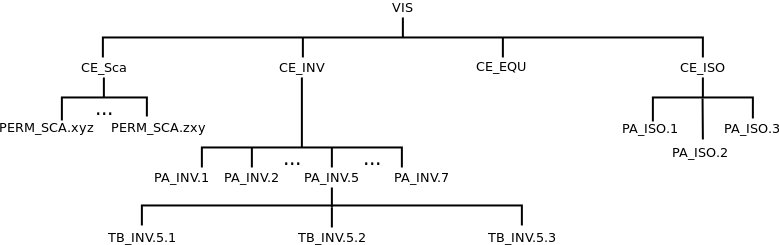
\includegraphics[scale=0.6]{\rootdir/ttf/figures/triangle-tth}
\caption{Test hierarchy for the Triangle program}
\label{fig:ttf:triangle-hierarchy}
\end{figure}

Note that at each node, the child nodes are all disjoint from each other, and the disjunction of the children nodes is equivalent to the parent node. 

These two properties are important, because if we know this holds for each parent-children relationship, then we can infer that following two facts:

\begin{enumerate}

 \item All leaf nodes are disjoint.

 \item The disjunction of all leaf nodes is equivalent to the valid input space.

\end{enumerate}

Therefore, we have a complete partition of the input space into disjoint tests.

\subsubsection*{Test templates}

To come up with tests, we take an entire path from the root node to a leaf node, and expand this.  For example, consider the leaf node \texttt{PERM\_SCA\_xyz}, defined as:

\begin{tabular}{lll}
         & \verb+PERM_SCA.xyz == [CE_SCA | x < y < z]+
\end{tabular}

This can be expanded as follows:

\begin{tabular}{lll}
         & \A/[CA_SCA | x < y < z]/\\[2mm]
$\equiv$ & \A/[VIS_Tri | validTriangle[x, y, z] and/\\
         & \A/            #(x+y+z) = 3 and x < z < y]/\\[2mm]
$\equiv$ & \A/[x, y, z : Int | validTriangle[x, y, z] and/\\
         & \A/            #(x+y+z) = 3 and x < z < y]/
\end{tabular}

Thus, following a path through the tree is the same as expanding the included predicates.

This is known as a \emph{test template}: it specifies the important properties of the test --- that is, the triangle is valid, and has three distinct sides such as \verb+x < y < z+, but it does not give specific values for tests. 

Tracing the path up the hierarchy helps to define the \emph{purpose} of this test template. By including the tactic names in the predicate names, this further helps to identify why each partition was done.

Importantly, this test template is simply equivalent to the Alloy predicate:

\lstset{aboveskip=3mm}
\alloyfile{linerange={30-34}}{\rootdir/ttf/models/triangle.als}


\subsection{Pruning infeasible paths}

Test templates are derived by taking all the leaf nodes of the test template hierarchy and conjoining the predicates along the path. However, some conjunctions can result in infeasible paths. Such infeasible paths must be removed, or {\em pruned}, from the hierarchy/tree.


For example, consider an alternate test hierarchy for the Triangle program in which there is a path \texttt{CE\_INV} $\rightarrow$ \texttt{PA\_INV.1} $\rightarrow$ \texttt{TB\_INV.1.2}, in which \texttt{TB\_INV.1.2} is the type-based partition:

\quad \verb|x = 0 and y = 0 and z != 0|.

Such a path would be infeasible because the only values that \verb+x,y,+ and \texttt{z} can take on to satisfy \texttt{PA\_INV.1}, which is:

\quad \verb|x >= y + z and y >= x + z and z >= x + y|

 is 

\quad \verb|x = y = z = 0|.

However, \verb|z = 0| is inconsistent with \verb|z != 0| above, so this path is infeasible. It is for this reason that we did not apply the TB tactic to this path in the running example. Had we chosen to apply it, we would now \emph{prune} this path from the tree.

Fortunately, we can check whether a test is infeasible using Alloy. The test template  \texttt{TB\_INV.1.2} is equivalent to the Alloy predicate:

\lstset{aboveskip=3mm}
\alloyfile{linerange={42-46}}{\rootdir/ttf/models/triangle.als}

By running the query:

\lstset{aboveskip=3mm}
\alloyfile{linerange={47-47}}{\rootdir/ttf/models/triangle.als}

we ask Alloy to try to find an instance for this. If it cannot, it means the predicate may be infeasible. The term \A+expect 0+ means that we expect this check to fail, so Alloy will not report the failure as an error.


\subsection{Deriving test cases}

Given a collection of test templates that describe sets of test cases, we need to derive specific instances of these to supply as actual test cases.

As an example, consider the path ending with the leaf node \texttt{PERM\_SCA.xyz} that is expanded above. This does not provide us with tests that can be run on an implementation of our triangle program, because it does not provide actual values for the test inputs. Instead, we need to select tests from this space.

The careful reader may have already determined how was can do this. We can use Alloy!

Given our test template definition, we need to just conjoin it with  with the operation under test and ask Alloy to solve an instance. For example, the corresponding predicate and run command for the \texttt{PERM\_SCA\_xyz} operation is:

\lstset{aboveskip=3mm}
\alloyfile{linerange={36-40}}{\rootdir/ttf/models/triangle.als}

Running the query will generate not only test inputs, but also an expected output for that input:

\begin{alloy}
skolem $PERM_SCA_xyz_x={4}
skolem $PERM_SCA_xyz_y={6}
skolem $PERM_SCA_xyz_z={5}
skolem $PERM_SCA_xyz_class={Scalene$0}
\end{alloy}

That is, \A+x = 4, y = 6, y = 5+ are the inputs, and \A+Scalene+ is the expected output.

This is a powerful tool. If we describe our test template as Alloy predicates, then we need to just conjoin the test template with the operation under test, and Alloy will generate one (or more!) test cases that satisfy the test template.

\begin{comment}
For this, the test templates must be instantiated to give {\em instance templates}.

\begin{definition}[Instance template]
Let \verb+TT_OP == [x+$_1$\verb+ : T+$_1$\verb+; +\ldots\verb+; x+$_n$\verb+ : +T$_n$\verb+ | P]+ be an expanded test template (leaf node) for an operation \texttt{Op}. An instance template for the test template \verb+TT_OP+ defined as:

\lstset{aboveskip=3mm}
\begin{alloy}[escapeinside={++}]
 IT_TT_OP == [TT_OP | x+$_1$+ = v+$_1$+ and + \ldots+ and x+$_n$+ = v+$_n$+]+
\end{alloy}

where \verb+v+$_1$, \ldots, \verb+v+$_n$ are constant values for the variables \verb+x+$_1$\verb+ : T+$_1$\verb+; +\ldots\verb+; x+$_n$\verb+ : +T$_n$ that satisfy the predicate \texttt{P}.
\end{definition}

\begin{example}~

Consider the test template \verb+PERM_SCA.xyz+ above. The following instance template instantiates the test template:

\lstset{aboveskip=3mm}
\lstset{language=}
\begin{alloy}
 IT1_PERM_SCA.xyz == [PERM_SCA.xyz | x = 2 and y = 3 and z = 4]
\end{alloy}
\end{example}

Again, we use this notation to both make our derivation neat, but also to document where the test came from. Therefore, from this instance template, we can see the purpose of the test by tracing back through the hierarchy.

\subsection{Deriving expected outputs}

Test derivation does not stop at inputs. For systematic testing, expected outputs are also important concepts. Unsurprisingly, to derive and document expected outputs, we extend the test template concept to produce \emph{oracle templates}. The TTF definition is particularly nice, because a general definition of an oracle template can be used, and then we solve the description to get the expected outputs.

\begin{definition}[Oracle template]
For an instance template \texttt{IT\_OP} of an operation \texttt{OP}, the corresponding oracle template is defined as:

\lstset{aboveskip=3mm}
\lstset{language=}
\begin{alloy}[escapeinside={++}]
 OT_OP == (OP and IT_OP) \ (x+$_1$, \ldots+ x+$_n$+)+
\end{alloy}

in which \verb+x+$_1$ \ldots\verb+x+$_n$ are the input and non-primed variables in \texttt{OP}, and \verb+\+ is the \emph{variable hiding} operator. The variable hiding operator removes, from the predicate, all variables in the brackets. Therefore, the oracle template is the solution for \texttt{OP} given inputs \texttt{IT\_OP}, but with only the output and primed variables remaining.

\end{definition}

\begin{example}
The oracle template for the \verb+IT1_PERM_SCA.xyz+ instance template is defined as:

\begin{tabular}{lll}
   & \verb+OT1_PERM_SCA.xyz == (Tri and IT1_PERM_SCA.xyz) \ (x, y, z)+
\end{tabular}

If we expand the conjunction, we get:

\begin{tabular}{lll}
  & \verb+[x, y, z : Int; class : Triangle |+\\
  & \verb+    validTriangle[x, y, z] and+\\
  & \verb+    #(x+y+z) = 1 <=> class = EQU and +\\
  & \verb+    #(x+y+z) = 2 <=> class = ISO and +\\
  & \verb+    #(x+y+z) = 3 <=> class = SCA and +\\
  & \verb+    x = 2 and y = 3 and z = 4] \ (x, y, z)+
\end{tabular}

Because this contains \verb+x = 2 and y = 3 and z = 4+, we know that the triangle is valid, and that \verb+#(x+y+z) = 3+, and therefore \verb+class = SCA+. This allows us to reduce this to the following:

\begin{tabular}{lll}
 & \verb+[x, y, z : Int; class : Triangle |+\\
 & \verb+    class = SCA and x = 2 and y = 3 and z = 4] \ (x, y, z)+
\end{tabular}

By applying the hiding operator, the final oracle template is:

\begin{tabular}{lll}
 & \verb+OT1_PERM_SCA.xyz == [class : Triangle | class = SCA]+
\end{tabular}

Therefore, by conjoining the original operation and the instance template, then solving the predicate and hiding the input variables, we end up with a template that describes the expected output.
\end{example}
\end{comment}

\subsubsection{Overview}

We briefly cap the process followed above, now that we have discussed each step.

First, we identified the input space and valid input space. Then, we apply test tactics to partition in the valid input space into a disjoint set of test templates, which can be represented as a hierarchy. The hierarchy helps to document the purpose of the test templates, and their corresponding tests. Test templates are then conjoined with the operation under test, and Alloy is used to generate complete test cases for the operation that satisfy the test template.


\section{Automation}

Throughout this chapter, we have demonstrated the application of the test template framework on a trivial example. Even then, we did not complete the example, because we left some templates unspecified to improve readability, and also did not apply certain tactics; e.g. boundary-value analysis to the scalene triangle example. 

Despite this, the hierarchy is already large and cumbersome, even for just a small example. For this to work in real software engineering, automation is required. Because our model is formal, we can apply many of the steps automatically.

The \emph{Fastest} tool \footnote{See \url{http://www.flowgate.net/?lang=en&seccion=herramientas}.} supports semi-automated application of the TTF. Fastest takes a Z specification and a set of tactics (implemented as Java classes) and applies these tactics exhaustively to produce a test template hierarchy. Then, it uses a constraint solver to automatically generate instance templates from the test templates, as well as to automatically generate the oracle templates for those instance templates. Fastest was derived and is maintained by Flowgate Consulting, who use it as part of their core business.

Utting and Legeard \cite{utting07} overview some of the most mature model-based testing tools and frameworks. While none of these implement the test template framework, they are all based on the same idea of partitioning. The test template framework laid the groundwork for many of these tools, including Microsoft's SpecExplorer model-based testing tool\footnote{See \url{http://research.microsoft.com/en-us/projects/specexplorer/}.}, which is used internally by several of Microsoft's product groups to test all of their APIs, and other companies such as Siemens.

Smartesting\footnote{See \url{http://www.smartesting.com/}.} are a French company specialising in model-based testing. Their tool set supports models in several different notations, include UML statecharts, and automatically generates test inputs and outputs on these. Their tools are founded on the test template framework, and incorporate constraint solving and AI search techniques to efficiently search out sequences of tests.

\section{Further reading}

The authoritative textbook on this is Utting and Legeard's  \cite{utting07} \emph{Practical Model-based Testing}. This textbook presents several model-based testing approaches and tools, and discusses industrial application of these. An electronic copy is available via the University of Melbourne library.





% LocalWords:  lifecycle hoc statecharts Glenford aboveskip linerange
% LocalWords:  validTriangle TTF Smartesting's toolset VIS dec pred
% LocalWords:  Tri ValidCase EQU SCA INV DNF disjuncts xyz xzy yxz eN
% LocalWords:  yzx zyx zxy ISE BVA TT Flowgate Utting Legeard pre lll
% LocalWords:  SpecExplorer Smartesting Legeard's versa APIs unary De
% LocalWords:  testability artifacts disjunction infeasible skolem
